\chapter{Hardware Used in Estimation}

\chapauthor{Darrel J. Conway}{Thinking Systems, Inc.}

GMAT's measurement models perform the task of calculating measurement values,
measurement derivatives, and associated properties of measurements needed for
estimation.  Many models depend on the physical characteristics of the hardware
that gathers the measurement data.  These characteristics are contained in the
hardware classes described in this chapter.

\section{Hardware Classes}

\begin{figure}[htbp]
\begin{center}
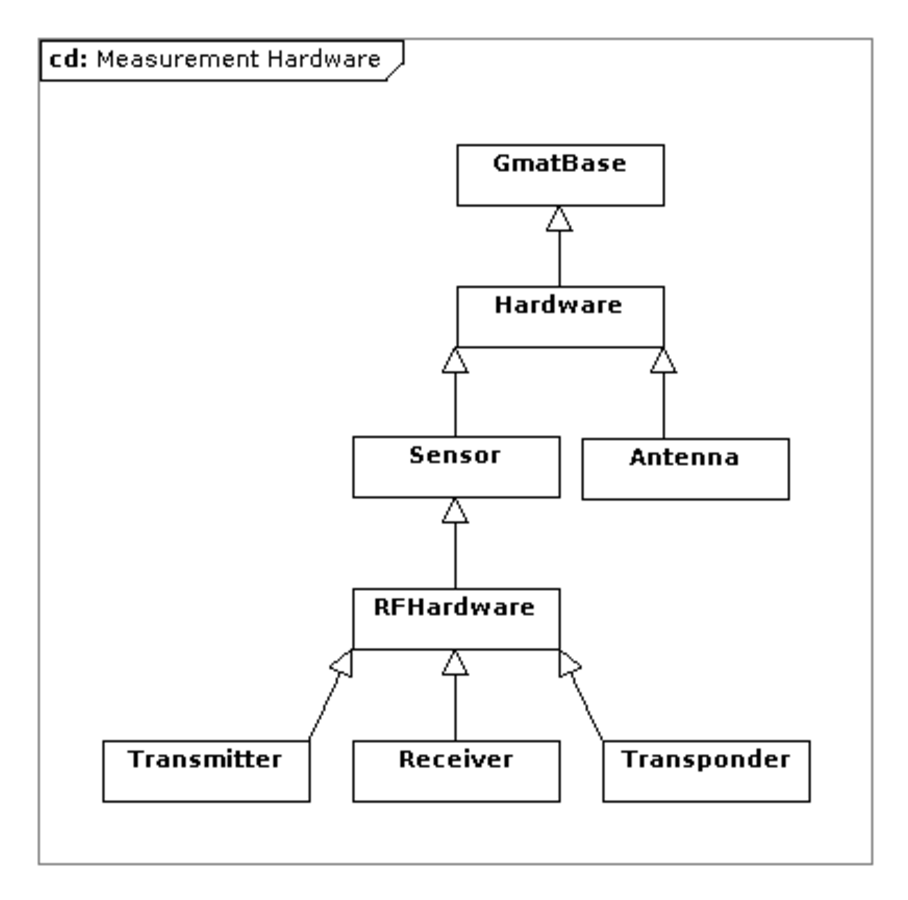
\includegraphics[scale=0.6]{Images/MeasurementHardware.eps}
% MeasurementHardware.png: 420x416 pixel, 72dpi
\caption{\label{fig:MeasurementHardware}Hardware Classes Used in Measurement
Modeling}
\end{center}
\end{figure}

\section{Estimation Interfaces}

The estimation subsystem accesses the properties and computations in the
hardware classes through a set of intefaces defined below.  The subsystem used
these interfaces to 
\begin{enumerate}
 \item \label{hw:feasibility}Evaluate signal based feasibility for a measurement
 \item \label{hw:delay}Find hardware associated delay values
 \item \label{hw:transmit}Retrieve signal properties for transmitters
 \item \label{hw:receive}Report signal properties to receivers
\end{enumerate}
\noindent
Many sensors modeled in GMAT's estimation processes have signal feasibility
constraints beyond simple line-of-sight constraints.  For example, receivers are
often constrained to specific frequency bands and optical sensors to specific
signal strengths before a measurement can be recorded.  The feasibility
interfaces (item~\ref{hw:feasibility}, above) captures these constraints. 
Detailed modeling requires that GMAT account for delays induced by electronics
in the hardware.  These delays are accessed using the interfaces supporting
item~\ref{hw:delay}.  Finally, the signal properties of transmitters need to be
accessed and passed into the signal receivers, potentially after modification
based on the signal propagation between the components.  These properties are
accessed through the transmitter and receiver interfaces,
items~\ref{hw:transmit} and~\ref{hw:receive}.

The methods supporting the estimation interfaces are defined in the Sensor
class.  The estimation hardware classes override these methods to implement the
sensor specific implementations of the methods.  GMAT's estimation subsystem
calls these interfaces to retrieve the data needed to calculate measurements and
their derivatives.  These measurement calculations are then used in the
simulation process to generate simulated measurements, or in the estimation
process to calculate the expected value of a measurement associated with teh
estimation hardware.

The following paragraphs define the interfaces that GMAT's estimation subsystem
uses for these processes.  We'll begin with a description of each method
defined fir this use in Sensor, and conclude with some representative overviews
of estimation processes that use these interfaces.

